\documentclass[11pt]{report}
\usepackage{fancyhdr}
\usepackage[usenames,dvipsnames,svgnames,table]{xcolor}
\usepackage[utf8]{inputenc}
\usepackage{setspace}
\usepackage{url}
\usepackage{hyperref}
\usepackage{float}
\usepackage{graphicx}
\usepackage{listings}
\usepackage{mips}
%tikz stuff
\usepackage{tikz}
\usetikzlibrary{shapes,shadows,arrows,backgrounds,positioning}
\tikzstyle{box1}=[rectangle, fill=orange!40, text width=1.5cm, rounded corners, text centered,font=\scriptsize, drop shadow]
\tikzstyle{box2}=[rectangle, fill=brown!40, text width=1.5cm, rounded corners, text centered,font=\scriptsize, drop shadow]
\tikzstyle{box3}=[rectangle, fill=gray!40, text width=1.5cm, rounded corners, text centered,font=\scriptsize, drop shadow]
\tikzstyle{box4}=[rectangle, fill=pink!90, text width=1.5cm, rounded corners, text centered,font=\scriptsize,drop shadow]
\tikzstyle{box5}=[rectangle, fill=orange, text width=1.5cm, minimum height=1.2cm, rounded corners, text centered,font=\scriptsize,drop shadow]
%tikz stages
\tikzstyle{stage}=[rectangle, fill=black!90, text=white, rounded corners, text width=1.5cm, text centered,font=\scriptsize,drop shadow]
\tikzstyle{stage2}=[rectangle, fill=black!10, text=black, rounded corners, text width=1.5cm, text centered,font=\scriptsize,drop shadow]
\tikzstyle{stage3}=[rectangle, fill=black!90, text=white, rounded corners, text width=6cm, text centered,font=\scriptsize,drop shadow]
%tikz arrow
\tikzstyle{arrow1}=[single arrow,draw=none, scale=1,minimum height=1cm, fill=red, drop shadow]
\tikzstyle{arrow2}=[single arrow,draw=none, scale=1,minimum height=1cm, fill=blue, drop shadow]
\tikzstyle{arrow3}=[single arrow,draw=none, scale=1,minimum height=1cm, fill=green, drop shadow]
\tikzstyle{arrow4}=[single arrow,draw=none, scale=1,minimum height=1cm, fill=green, rotate=-60, drop shadow]
\tikzstyle{arrow5}=[single arrow,draw=none, scale=1,minimum height=1cm, fill=green, rotate=60, drop shadow]
%tikz stuff end

\definecolor{mygreen}{rgb}{0,0.6,0}
\definecolor{mygray}{rgb}{0.5,0.5,0.5}
\definecolor{mymauve}{rgb}{0.58,0,0.82}

\lstset{ %
  backgroundcolor=\color{white},   % choose the background color; you must add \usepackage{color} or \usepackage{xcolor}
  basicstyle=\footnotesize,        % the size of the fonts that are used for the code
  breakatwhitespace=false,         % sets if automatic breaks should only happen at whitespace
  breaklines=true,                 % sets automatic line breaking
  captionpos=b,                    % sets the caption-position to bottom
  commentstyle=\color{mygreen},    % comment style
  deletekeywords={...},            % if you want to delete keywords from the given language
  escapeinside={\%*}{*)},          % if you want to add LaTeX within your code
  extendedchars=true,              % lets you use non-ASCII characters; for 8-bits encodings only, does not work with UTF-8
  frame=single,                    % adds a frame around the code
  keepspaces=true,                 % keeps spaces in text, useful for keeping indentation of code (possibly needs columns=flexible)
  keywordstyle=\color{blue},       % keyword style
  language=Octave,                 % the language of the code
  morekeywords={*,...},            % if you want to add more keywords to the set
  numbers=left,                    % where to put the line-numbers; possible values are (none, left, right)
  numbersep=5pt,                   % how far the line-numbers are from the code
  numberstyle=\tiny\color{mygray}, % the style that is used for the line-numbers
  rulecolor=\color{black},         % if not set, the frame-color may be changed on line-breaks within not-black text (e.g. comments (green here))
  showspaces=false,                % show spaces everywhere adding particular underscores; it overrides 'showstringspaces'
  showstringspaces=false,          % underline spaces within strings only
  showtabs=false,                  % show tabs within strings adding particular underscores
  stepnumber=2,                    % the step between two line-numbers. If it's 1, each line will be numbered
  stringstyle=\color{mymauve},     % string literal style
  tabsize=2,                       % sets default tabsize to 2 spaces
  title=\lstname                   % show the filename of files included with \lstinputlisting; also try caption instead of title
}

\usepackage[backend=biber,
style=authoryear-comp,
natbib=true,
]{biblatex}
\usepackage{titlesec}
\titleformat*{\section}{\Large\bfseries\sffamily\color{Sepia}}
\titleformat*{\subsection}{\large\bfseries\sffamily\color{Bittersweet}}
\titleformat*{\subsubsection}{\large\bfseries\sffamily\color{RedOrange}}
\addbibresource{JNMansfield-CS440-ARM11-Report.bib}
\begin{document}
\lstset{language=[mips]Assembler}
\begin{titlepage}

\begin{center}
\textsc{{\LARGE\color{Sepia}{CS440}}}\\[1.5cm]
\textsc{{\LARGE\color{Bittersweet}{ARM11}}}\\[1.5cm]

\begin{minipage}{0.4\textwidth}
\begin{flushleft} \large
\emph{\color{RedOrange}{Author}:}\\
Mr. Jason \textsc{Mansfield}
\end{flushleft}\end{minipage}
\begin{minipage}{0.4\textwidth}
\begin{flushright} \large
\emph{\color{RedOrange}Instructor:} \\
Prof.~Pamela~\textsc{Smallwood}
\end{flushright}
\end{minipage}
\end{center}
\end{titlepage}

\tableofcontents
\clearpage
\section{In the beginning there was Acorn}
\begin{doublespace}
In 1985 the first ARM processor, the Acorn RISC Machine was introduced to the world~\citep{levy2005history}. Later in 1990 the Advanced RISC Machines Ltd.(ARM) would be launched. Unlike other RISC processor vendors of their time ARM began creating small scale processors. A whitepaper~\citep{kamath2001system} from 2001 Strategy made this statement: 
\end{doublespace}
\begin{quote}
At Wipro, significant focus has been on the ARM processor technology, since we believe that will drive the evolving market for embedded applications, mobile devices and next generation information appliances.
\end{quote}
\begin{doublespace}
Although this insight was probably not difficult to gauge by 2001, the scale at which embedded mobile devices has exploded onto the market has been impressive. Larger corporations, which have not been know for ingenuity, such as Microsoft, have been dealt a massive blow by new mobile devices such as Apples IOS based iPhone and iPad, or the fleets of Android based devices. The need for a smaller architecture has never been greater and ARM is sitting center stage. 
\end{doublespace}
\subsection{The need for a smaller silicon area}
\begin{doublespace}
The ARM architecture a \textbf{Reduced Instruction Set Computer} or RISC based architecture is now considered a dominant choice for developers and manufacturers. The ARM architecture incorporates standard RISC features~\citep[A1-2]{referenceB}:
\end{doublespace}

\begin{itemize}
\item a large uniform register file.
\item a load/store architecture, where data-processing operations only operate on register contents, not directly on memory contents.
\item simple addressing modes, with all load/store addresses being determined from register contents and instruction fields only.
\end{itemize}
\begin{doublespace}
The ARM architecture has proven to be a better choice for smaller devices due to the low power consumption along with good performance. The \textbf{RM Architecture Reference Manual} listed the following additional reasons ARM is designed for smaller devices~\citep[A1-2]{referenceB}:
\end{doublespace}
\begin{itemize}
\item instructions that combine a shift with an arithmetic or logical operation.
\item auto-increment and auto-decrement addressing modes to optimize program loops.
\item Load and Store Multiple instructions to maximize data throughput.
\item conditional execution of almost all instructions to maximize execution throughput.
\end{itemize}
\section{The Instruction Set Architecture}
Currently ARMv6 has ISA support for the following~\citep{ARM1176}:
\begin{itemize}
\item ARM
\item Thumb\textregistered
\item Jazelle DBX\textregistered
\item DSP extension
\item Floating Point Unit
\end{itemize}
\begin{doublespace}
\subsection{state switching}
The ARM processor allows switching of states using the BX and BLX instructions. The ARM state is 32-bit word-aligned, the Thumb a 16-bit halfword-aligned, and the Jazelle state is variable length, byte aligned for instructions~\citep[2-12]{arm1176jzf-s}.
\end{doublespace}
\subsection{A32}
\begin{doublespace}
ARM is also known as A32~\citep{A32}. ARMv6 architecture is amongst a few others which use A32 such as ARMv5TEJ and ARMv4T. 
\subsubsection{ Instruction length and format}
ARM instructions are 32-bits wide and have a 4-byte boundary~\citep{A32}. The subdivisions of the ARM instruction set can be seen in the below figure 1~\citep[A5-2]{referenceB}. As you can see each ARM instruction is composed of a 32-bit word. The 32-bit word's subdivisions are determined by bits [31:25,4]. Additionally, the conditional subdivision can be see between bits [31:28]. The conditional field allows for more optimizations.
\end{doublespace}

\begin{center}
\rowcolors{1}{gray!10}{brown!10}
\begin{figure}[H] 
\resizebox{\textwidth}{!}{%
\begin{tabular}{|c|c|c|c|c|c|c|}
\hline
31~30~29~28& 27~26~25 & 24~23~22~21~20~19~18~17~16~15~14~13~12~11~10~9~8~7~6~5& 4 & 3~2~1~0\\
\hline
cond & op1 &  & op & \\ \hline
\end{tabular}}
\caption{ARM subdivisions}
\end{figure}
\end{center}
\subsubsection{General Instruction Categories}
\begin{doublespace}
The following figure 2, shown below, illustrates the encoding which defines the various classes of instructions used with ARMv6~\citep[A5-2]{referenceB}:
\end{doublespace}

\begin{center}
\rowcolors{1}{gray!10}{brown!10}
\begin{figure}[H] 
\resizebox{\textwidth}{!}{%
\begin{tabular}{|c|c|c|c|}
\hline
cond & op1 & op & Instruction classes\\ \hline \hline
not 1111 & 00x & - & Data-processing and misc instructions\\ \hline
not 1111 & 010 & - & Load/Store word and unsigned byte\\ \hline
not 1111 & 011 & 0 & Load/Store word and unsigned byte\\ \hline
not 1111 & 011 & 1 & Media instructions\\ \hline
not 1111 & 10x & - & Branch, branch with link, and block data transfer\\ \hline
not 1111 & 11x & - & Supervisor Call and coprocessor instructions\\ \hline \hline
1111 & - & - & Unconditionally executed\\ \hline
\end{tabular}}
\caption{ARM Instruction encoding}
\end{figure}
\end{center}
\subsubsection{The Branch Instruction}
\begin{doublespace}
As can be seen in figure 2 op1 determines the instruction class. For example when op1 = 10x one of the various branching or block data transfer instructions is being used. If branch is the instruction specifically being used then 10xxxx will be found between [25:20] as shown in figure 3 below~\citep[A5-27]{referenceB}: 
\end{doublespace}

\begin{center}
\rowcolors{1}{gray!10}{brown!10}
\begin{figure}[H] 
\resizebox{\textwidth}{!}{%
\begin{tabular}{|c|c|c|c|c|c|c|}
\hline
31~30~29~28& 27~26 & 25~24~23~22~21~20 & 19~18~17~16& 15 & 14~13~12~11~10~9~8~7~6~5~4~3~2~1~0\\
\hline
cond & 1~0 & op &  &  &   \\ \hline
not 1111 & 1~0 & 10xxxx &  & &\\ \hline
\end{tabular}}
\caption{Branch equals 10xxxx}
\end{figure}
\end{center}
\begin{doublespace}
Going a step further, the following figure 4 shows the branch instructions details in Encoding A1~\citep[A8-44]{referenceB}.
\end{doublespace}
\begin{center}
\rowcolors{1}{gray!10}{brown!10}
\begin{figure}[H] 
\resizebox{\textwidth}{!}{%
\begin{tabular}{|c|c|c|}
\hline
31~30~29~28& 27~26~25~24 & 23~22~21~20~19~18~17~16~15~14~13~12~11~10~9~8~7~6~5~4~3~2~1~0\\
\hline
cond & 1~0~1~0& imm24   \\ \hline
\end{tabular}}
\caption{imm32 = SignExtend(imm24:'00', 32);}
\end{figure}
\end{center}
\begin{doublespace}
Encoding A1 indicates multiples of 4 in the range $-33554432$ to $33554428$. Other encodings such as T1, T2, T3, and T4 have smaller ranges with T1 being the smallest of the permitted offsets. The T1 range is $-256$ to $254$. All other offset ranges besides Encoding A1 are in even numbers, while Encoding A1, shown in figure 4, is in Multiples of 4. ARM encodings are labeled as A1, A2, A3 and so forth, while Thumb encodings are listed as T1, T2, T3 and so forth. Additionally, there are also encodings for ThumbEE which are listed as E1, E2, E3 and so forth~\citep[A8-282]{referenceB}. 
\end{doublespace}
\subsubsection{The MOV Instruction}
\begin{doublespace}
Looking back at figure 2 to op1 = 00x you can see the 27th and 26th bit is determined to be both 0 for all instructions defined as data processing and misc. 
\end{doublespace}
\begin{center}
\rowcolors{1}{gray!10}{brown!10}
\begin{figure}[H] 
\resizebox{\textwidth}{!}{%
\begin{tabular}{|c|c|c|c|c|c|c|}
\hline
31~30~29~28& 27~26 & 25 & 24~23~22~21~20 & 19~18~17~16~15~14~13~12~11~10~9~8 & 7~6~5~4 & 3~2~1~0\\
\hline
cond & 0~0 & op &op1  &  &op2 &  \\ \hline
\end{tabular}}
\caption{Data-processing and misc}
\end{figure}
\end{center}
\begin{doublespace}
One instruction which falls under the category of data processing is the MOV instruction. The following figure demonstrates the use of the MOV instruction in encoding A1~\citep[A8-194]{referenceB}. 
\end{doublespace}

\begin{center}
\rowcolors{1}{gray!10}{brown!10}
\begin{figure}[H] 
\resizebox{\textwidth}{!}{%
\begin{tabular}{|c|c|c|c|c|c|c|c|}
\hline
31~30~29~28& 27~26 & 25 & 24~23~22~21 & 20 & 19~18~17~16 & 15~14~13~12 & 11~10~9~8~7~6~5~4~3~2~1~0\\
\hline
cond & 0~0 & 1 & 1~1~0~1 & S & (0)(0)(0)(0) & Rd & imm12  \\ \hline
\end{tabular}}
\caption{MOV instruction}
\end{figure}
\end{center}
\subsection{Syntax for using the branch and mov instructions}
\begin{doublespace}
The aforementioned instructions mov and branch are used in the following manor: 
\end{doublespace}
\begin{lstlisting}
/*an assembly code example using instruction mov*/
.global main
.func main

main:
     mov r0, #11 /* Put the number eleven in register r0*/
     bx lr
\end{lstlisting}
\begin{doublespace}
The below code clip shows a unconditional branch being used:
\end{doublespace}
\begin{lstlisting}
/*an assembly code example using the unconditional branch instruction*/
.text
.global main
main:
      mov r0, #11
      b finish/*branch to finish*/
      mov r0, #22
finish:
      bx lr

\end{lstlisting}
\begin{doublespace}
When the above code is run the second mov instruction will be skipped due to the branch instruction pointing to \textit{finish}.
\end{doublespace}
\section{The main components of the ARM1176JZF-S}
\begin{doublespace}
The following components are considered the main components for the ARM1176JZF-S processor~\citep[1-8]{arm1176jzf-s}:
\subsection{List of components}
\end{doublespace}
\begin{description}
\item[Integer Core] The ARM1176JZF-S processor is built around the ARM11 integer core. Therefore, it is a implementation of the ARMv6 architecture. This architecture handles the following critical items~\citep[1-9]{arm1176jzf-s}:
\begin{itemize}
\item Instruction sets
\item Conditional execution
\item Registers
\item Modes and exceptions
\item Thumb instruction set
\item DSP instructions
\item Media extensions
\item Datapath
\item Branch prediction
\item Return Stack
\end{itemize}
\item[Load Store Unit (LSU)] The load-store pipeline decouples loads and stores from the MAC and ALU~\citep[1-11]{arm1176jzf-s}.
\item [Prefetch unit] Fetches instructions from the instruction cache, external memory and instruction TCM to predict branch outcomes~\citep[1-11]{arm1176jzf-s}.
\item [Memory system] The memory system provides the core with features such as virtual indexing, export of memory, memory access control and many other capabilities~\citep[1-12]{arm1176jzf-s}.
\item [AMBA AXI interface] This bus interface allows high bandwidth connectivity between the processor, second level caches, on-chip RAM, peripherals, and interfaces to external memory~\citep[1-16]{arm1176jzf-s}. 
\item [Coprocessor interface] This is a external coprocessor which interfaces with the ARM1176JZF-S to handle ARM coprocessor instructions~\citep[1-17]{arm1176jzf-s}.
\item [Debug] Using the ARMv6 debug architecture the following levels of debugging are allowed~\citep[1-18]{arm1176jzf-s}:
\begin{itemize}
\item debug everywhere
\item debug in non-secure privileged user, and secure user.
\item debug in non-secure.
\end{itemize}
\item [Instruction cycle summary and interlocks] Allows handling of cycle timing behavior.
\item [Vector Floating-Point (VFP)] Handles floating point arithmetic operations~\citep[1-19]{arm1176jzf-s}.
\item [System control] Controls the memory system and other functionality~\citep[1-21]{arm1176jzf-s}.
\item [Interrupt handling] The interrupt handling deal with the following areas~\citep[1-21]{arm1176jzf-s}:
\begin{itemize}
\item Vectors Interrupt Controller port
\item Low interrupt latency configuration
\item Configuration
\item Exception processing enhancements
\end{itemize}
\end{description}
\section{ARM1176JZF-S pipeline stages}
\begin{doublespace}
The ARM1176JZF-S  processor overlaps operations to improve clock rate speed for each instruction. For the following figures 7-12 note that the first 4 stages Fe1, Fe2, De, Iss are considered the \textbf{common decode pipeline}. From the common decode pipeline the direction taken will determine if the instruction will seek a ALU pipeline, Multiply pipeline, or a Load/Store pipeline. 
\end{doublespace}

\begin{figure}[H]
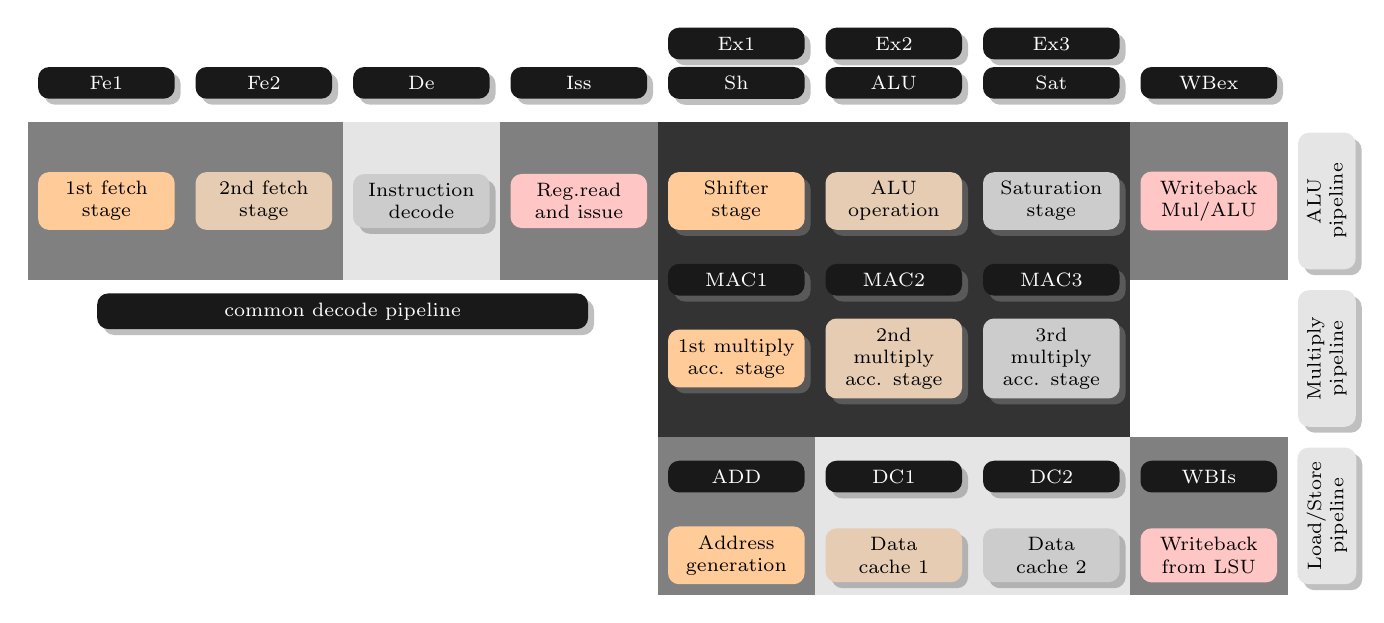
\begin{tikzpicture}

%Row One
\node[stage2,rotate=90](alup) at (7.5,0){ALU pipeline};
\node[stage2,rotate=90](mulp) at (7.5,-2){Multiply pipeline};
\node[stage2,rotate=90](lsp) at (7.5,-4){Load/Store pipeline};
\node[stage3](cdp) at (-5,-1.4){common decode pipeline};
\node[stage] (s1) at (-8,1.5){Fe1};
\node[box1] (bx1) at (-8,0){1st fetch stage};
\node[stage] (s) at (-6,1.5){Fe2};
\node[box2] (bx2) at (-6,0){2nd fetch stage};
\node[stage] (s3) at (-4,1.5){De};
\node[box3] (bx3) at (-4,0){Instruction decode};
\node[stage] (s4) at (-2,1.5){Iss};
\node[box4] (bx4) at (-2,0){Reg.read and issue};
\node[stage] (e1) at (0,2){Ex1};
\node[stage] (e2) at (2,2){Ex2};
\node[stage] (e3) at (4,2){Ex3};
\node[stage] (s5) at (0,1.5){Sh};
\node[box1] (bx5) at (0,0){Shifter stage};
\node[stage] (s6) at (2,1.5){ALU};
\node[box2] (bx6) at (2,0){ALU\\operation};
\node[stage] (s7) at (4,1.5){Sat};
\node[box3] (bx7) at (4,0){Saturation stage};
\node[stage] (s8) at (6,1.5){WBex};
\node[box4] (bx8) at (6,0){Writeback Mul/ALU};
%Row Two
\node[stage] (s2_1) at (0,-1){MAC1};
\node[box1] (r2bx1) at (0,-2){1st multiply\\acc. stage};
\node[stage] (s2_2) at (2,-1){MAC2};
\node[box2] (r2bx2) at (2,-2){2nd multiply\\acc. stage};
\node[stage] (s2_3) at (4,-1){MAC3};
\node[box3] (r2bx3) at (4,-2){3rd multiply\\acc. stage};
%Row Three
\node[stage] (s3_1) at (0,-3.5){ADD};
\node[box1] (r3bx1) at (0,-4.5){Address generation};
\node[stage] (s3_2) at (2,-3.5){DC1};
\node[box2] (r3bx2) at (2,-4.5){Data cache 1};
\node[stage] (s3_3) at (4,-3.5){DC2};
\node[box3] (r3bx3) at (4,-4.5){Data cache 2};
\node[stage] (s3_4) at (6,-3.5){WBIs};
\node[box4] (r3bx4) at (6,-4.5){Writeback from LSU};
%background
\begin{scope}[on background layer]
\fill[black!50](-9,-1) rectangle(-5,1);
\end{scope}

\begin{scope}[on background layer]
\fill[black!10](-5,-1) rectangle(-3,1);
\end{scope}

\begin{scope}[on background layer]
\fill[black!50](-3,-1) rectangle(-1,1);
\end{scope}

\begin{scope}[on background layer]
\fill[black!80](-1,-3) rectangle(5,1);
\end{scope}

\begin{scope}[on background layer]
\fill[black!50](-1,-5) rectangle(1,-3);
\end{scope}

\begin{scope}[on background layer]
\fill[black!10](1,-5) rectangle(5,-3);
\end{scope}


\begin{scope}[on background layer]
\fill[black!50](5,-1) rectangle(7,1);
\end{scope}

\begin{scope}[on background layer]
\fill[black!50](5,-5) rectangle(7,-3);
\end{scope}

\end{tikzpicture}
\caption{ARM1176JZF-S pipeline stages}
\end{figure}
%begin ALU operation
\begin{figure}[H]
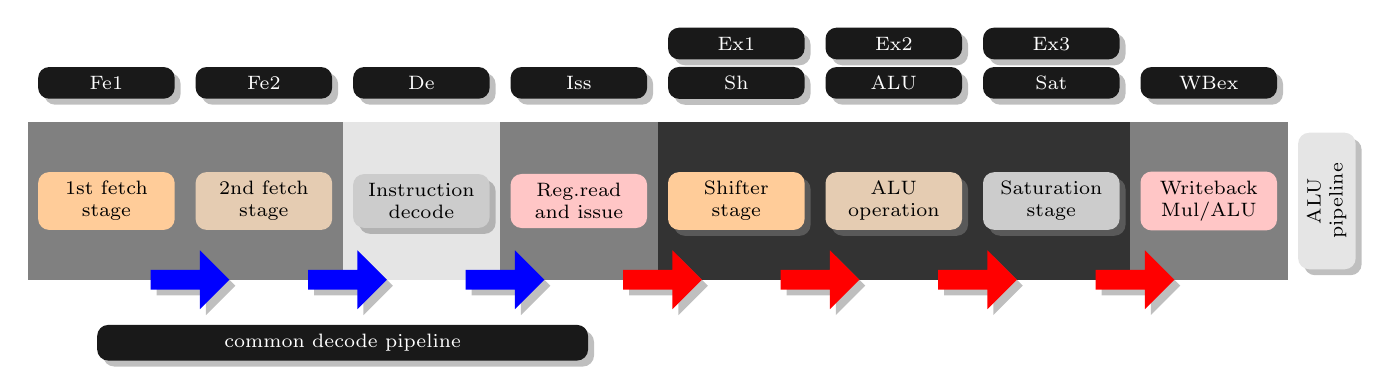
\begin{tikzpicture}
%Arrows
\node[arrow2](ar1) at (-7,-1){};
\node[arrow2](ar2) at (-5,-1){};
\node[arrow2](ar3) at (-3,-1){};
\node[arrow1](ar4) at (-1,-1){};
\node[arrow1](ar5) at ( 1,-1){};
\node[arrow1](ar6) at ( 3,-1){};
\node[arrow1](ar7) at ( 5,-1){};
%Row One
\node[stage2,rotate=90](alup) at (7.5,0){ALU pipeline};
\node[stage3](cdp) at (-5,-1.8){common decode pipeline};
\node[stage] (e1) at (0,2){Ex1};
\node[stage] (e2) at (2,2){Ex2};
\node[stage] (e3) at (4,2){Ex3};
\node[stage] (s1) at (-8,1.5){Fe1};
\node[box1] (bx1) at (-8,0){1st fetch stage};
\node[stage] (s) at (-6,1.5){Fe2};
\node[box2] (bx2) at (-6,0){2nd fetch stage};
\node[stage] (s3) at (-4,1.5){De};
\node[box3] (bx3) at (-4,0){Instruction decode};
\node[stage] (s4) at (-2,1.5){Iss};
\node[box4] (bx4) at (-2,0){Reg.read and issue};
\node[stage] (s5) at (0,1.5){Sh};
\node[box1] (bx5) at (0,0){Shifter stage};
\node[stage] (s6) at (2,1.5){ALU};
\node[box2] (bx6) at (2,0){ALU\\operation};
\node[stage] (s7) at (4,1.5){Sat};
\node[box3] (bx7) at (4,0){Saturation stage};
\node[stage] (s8) at (6,1.5){WBex};
\node[box4] (bx8) at (6,0){Writeback Mul/ALU};
%Row Two
%background
\begin{scope}[on background layer]
\fill[black!50](-9,-1) rectangle(-5,1);
\end{scope}

\begin{scope}[on background layer]
\fill[black!10](-5,-1) rectangle(-3,1);
\end{scope}

\begin{scope}[on background layer]
\fill[black!50](-3,-1) rectangle(-1,1);
\end{scope}

\begin{scope}[on background layer]
\fill[black!80](-1,-1) rectangle(5,1);
\end{scope}


\begin{scope}[on background layer]
\fill[black!50](5,-1) rectangle(7,1);
\end{scope}

\end{tikzpicture}
\caption{ARM1176JZF-S ALU Operation}
\end{figure}
%begin multiply operation
\begin{figure}[H]
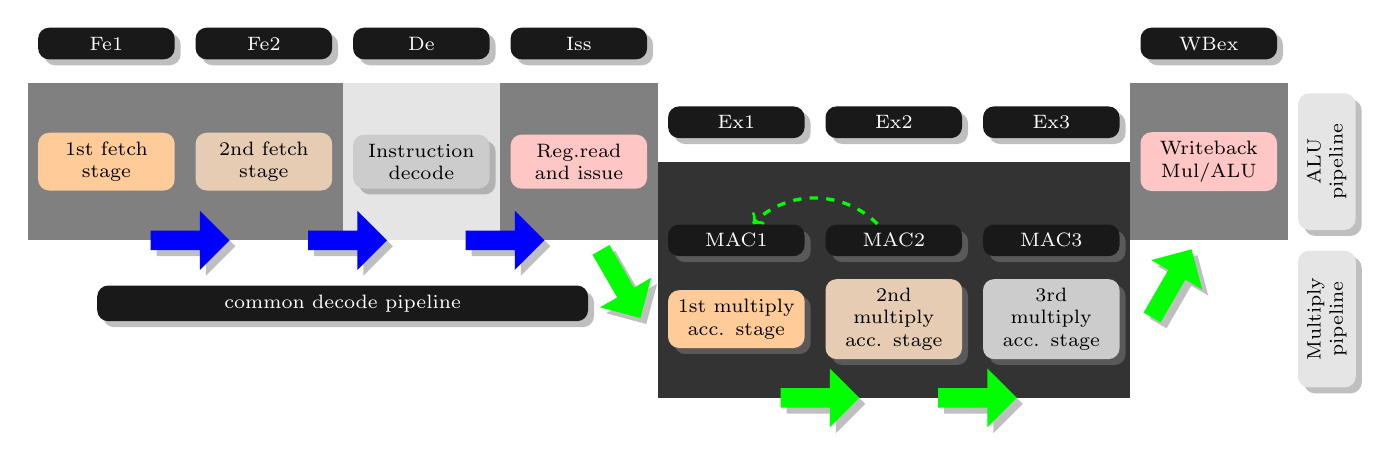
\begin{tikzpicture}
%Arrows
\node[arrow2](ar1) at (-7,-1){};
\node[arrow2](ar2) at (-5,-1){};
\node[arrow2](ar3) at (-3,-1){};
\node[arrow4](ar4) at (-1.5,-1.5){};
\node[arrow3](ar5) at (1,-3){};
\node[arrow3](ar6) at (3,-3){};
\node[arrow5](ar7) at (5.5,-1.6){};

%Row One
\node[stage2,rotate=90](alup) at (7.5,0){ALU pipeline};
\node[stage2,rotate=90](mulp) at (7.5,-2){Multiply pipeline};
\node[stage3](cdp) at (-5,-1.8){common decode pipeline};
\node[stage] (e1) at (0,.5){Ex1};
\node[stage] (e2) at (2,.5){Ex2};
\node[stage] (e3) at (4,.5){Ex3};
\node[stage] (s1) at (-8,1.5){Fe1};
\node[box1] (bx1) at (-8,0){1st fetch stage};
\node[stage] (s) at (-6,1.5){Fe2};
\node[box2] (bx2) at (-6,0){2nd fetch stage};
\node[stage] (s3) at (-4,1.5){De};
\node[box3] (bx3) at (-4,0){Instruction decode};
\node[stage] (s4) at (-2,1.5){Iss};
\node[box4] (bx4) at (-2,0){Reg.read and issue};
\node[stage] (s8) at (6,1.5){WBex};
\node[box4] (bx8) at (6,0){Writeback Mul/ALU};
%Row Two
\node[stage] (s2_1) at (0,-1){MAC1};
\node[box1] (r2bx1) at (0,-2){1st multiply\\acc. stage};
\node[stage] (s2_2) at (2,-1){MAC2};
\node[box2] (r2bx2) at (2,-2){2nd multiply\\acc. stage};
%arrow
\draw[->, color=green, very thick, dashed] (s2_2) to [bend right=45] (s2_1);
\node[stage] (s2_3) at (4,-1){MAC3};
\node[box3] (r2bx3) at (4,-2){3rd multiply\\acc. stage};
%background
\begin{scope}[on background layer]
\fill[black!50](-9,-1) rectangle(-5,1);
\end{scope}

\begin{scope}[on background layer]
\fill[black!10](-5,-1) rectangle(-3,1);
\end{scope}

\begin{scope}[on background layer]
\fill[black!50](-3,-1) rectangle(-1,1);
\end{scope}

\begin{scope}[on background layer]
\fill[black!80](-1,-3) rectangle(5,0);
\end{scope}

\begin{scope}[on background layer]
\fill[black!50](5,-1) rectangle(7,1);
\end{scope}


\end{tikzpicture}
\caption{ARM1176JZF-S Multiply Operation}
\end{figure}

%begin LDR/STR operation
\begin{figure}[H]
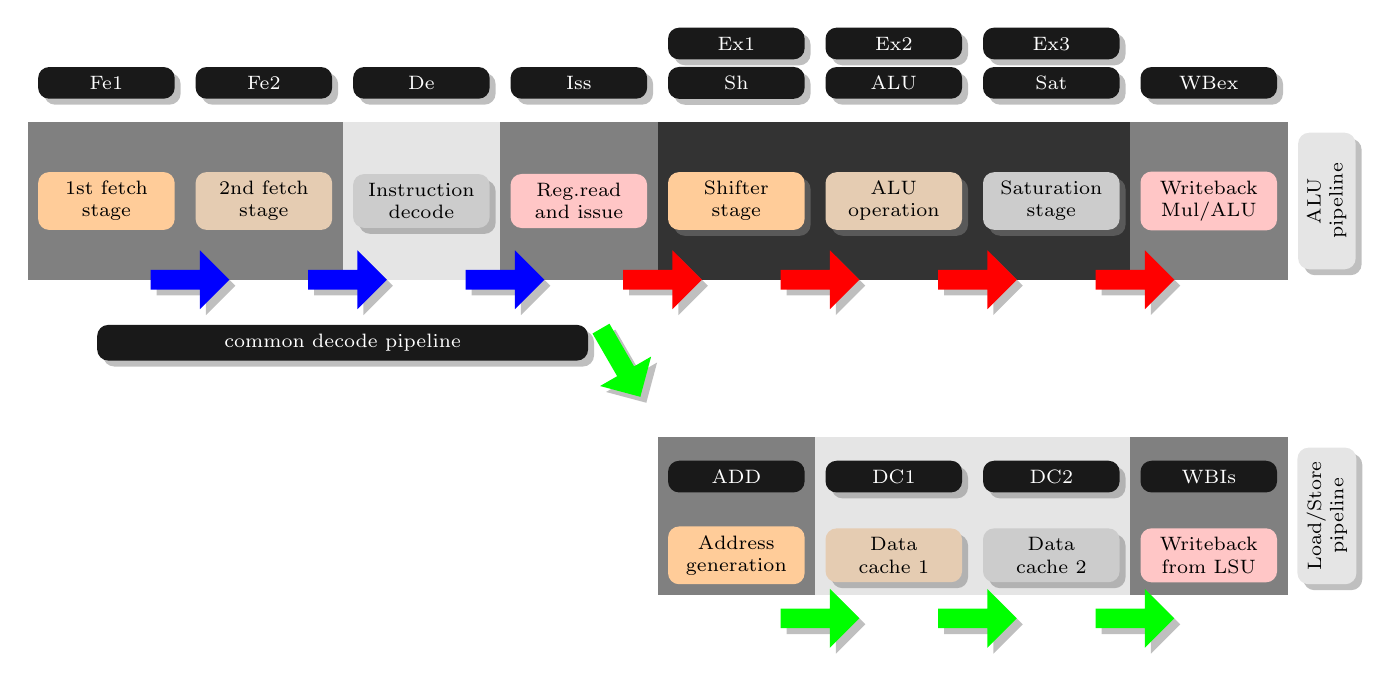
\begin{tikzpicture}
%Arrows
\node[arrow2](ar1) at (-7,-1){};
\node[arrow2](ar2) at (-5,-1){};
\node[arrow2](ar3) at (-3,-1){};
\node[arrow1](ar4) at (-1,-1){};
\node[arrow1](ar5) at ( 1,-1){};
\node[arrow1](ar6) at ( 3,-1){};
\node[arrow1](ar7) at ( 5,-1){};
\node[arrow4](ar8) at ( -1.5,-2){};
\node[arrow3](ar9) at (1,-5.3){}; 
\node[arrow3](ar9) at (3,-5.3){}; 
\node[arrow3](ar9) at (5,-5.3){}; 

%Row One
\node[stage2,rotate=90](alup) at (7.5,0){ALU pipeline};
\node[stage2,rotate=90](lsp) at (7.5,-4){Load/Store pipeline};
\node[stage3](cdp) at (-5,-1.8){common decode pipeline};
\node[stage] (e1) at (0,2){Ex1};
\node[stage] (e2) at (2,2){Ex2};
\node[stage] (e3) at (4,2){Ex3};
\node[stage] (s1) at (-8,1.5){Fe1};
\node[box1] (bx1) at (-8,0){1st fetch stage};
\node[stage] (s) at (-6,1.5){Fe2};
\node[box2] (bx2) at (-6,0){2nd fetch stage};
\node[stage] (s3) at (-4,1.5){De};
\node[box3] (bx3) at (-4,0){Instruction decode};
\node[stage] (s4) at (-2,1.5){Iss};
\node[box4] (bx4) at (-2,0){Reg.read and issue};
\node[stage] (s5) at (0,1.5){Sh};
\node[box1] (bx5) at (0,0){Shifter stage};
\node[stage] (s6) at (2,1.5){ALU};
\node[box2] (bx6) at (2,0){ALU\\operation};
\node[stage] (s7) at (4,1.5){Sat};
\node[box3] (bx7) at (4,0){Saturation stage};
\node[stage] (s8) at (6,1.5){WBex};
\node[box4] (bx8) at (6,0){Writeback Mul/ALU};
%Row Three
\node[stage] (s3_1) at (0,-3.5){ADD};
\node[box1] (r3bx1) at (0,-4.5){Address generation};
\node[stage] (s3_2) at (2,-3.5){DC1};
\node[box2] (r3bx2) at (2,-4.5){Data cache 1};
\node[stage] (s3_3) at (4,-3.5){DC2};
\node[box3] (r3bx3) at (4,-4.5){Data cache 2};
\node[stage] (s3_4) at (6,-3.5){WBIs};
\node[box4] (r3bx4) at (6,-4.5){Writeback from LSU};
%background
\begin{scope}[on background layer]
\fill[black!50](-9,-1) rectangle(-5,1);
\end{scope}

\begin{scope}[on background layer]
\fill[black!10](-5,-1) rectangle(-3,1);
\end{scope}

\begin{scope}[on background layer]
\fill[black!50](-3,-1) rectangle(-1,1);
\end{scope}

\begin{scope}[on background layer]
\fill[black!80](-1,-1) rectangle(5,1);
\end{scope}

\begin{scope}[on background layer]
\fill[black!50](-1,-5) rectangle(1,-3);
\end{scope}

\begin{scope}[on background layer]
\fill[black!10](1,-5) rectangle(5,-3);
\end{scope}


\begin{scope}[on background layer]
\fill[black!50](5,-1) rectangle(7,1);
\end{scope}

\begin{scope}[on background layer]
\fill[black!50](5,-5) rectangle(7,-3);
\end{scope}

\end{tikzpicture}
\caption{ARM1176JZF-S LDR/STR operation }
\end{figure}

%begin LDM/STM op
\begin{figure}[H]
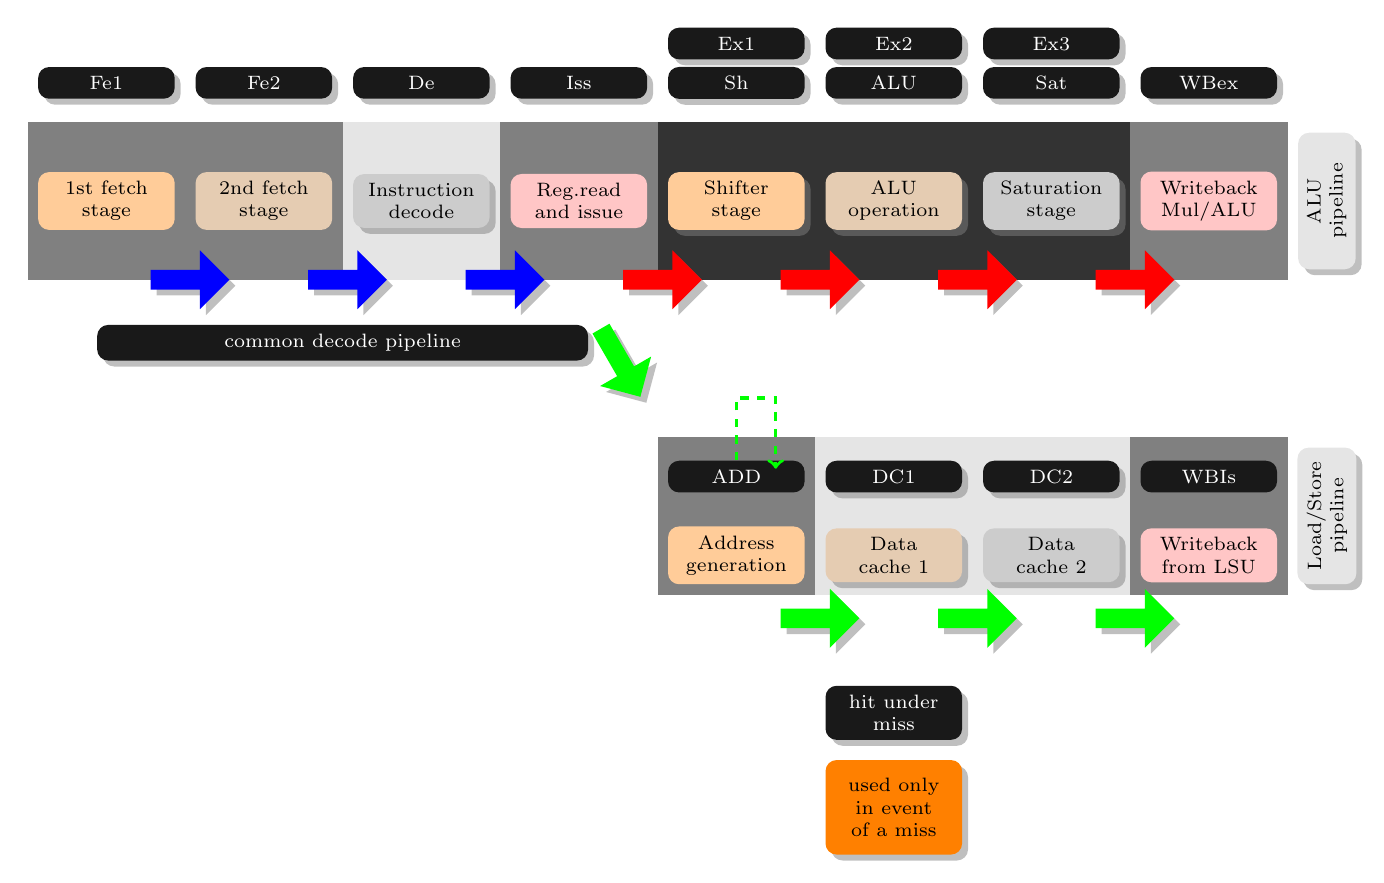
\begin{tikzpicture}
%Arrows
\node[arrow2](ar1) at (-7,-1){};
\node[arrow2](ar2) at (-5,-1){};
\node[arrow2](ar3) at (-3,-1){};
\node[arrow1](ar4) at (-1,-1){};
\node[arrow1](ar5) at ( 1,-1){};
\node[arrow1](ar6) at ( 3,-1){};
\node[arrow1](ar7) at ( 5,-1){};
\node[arrow4](ar8) at ( -1.5,-2){};
\node[arrow3](ar9) at (1,-5.3){}; 
\node[arrow3](ar9) at (3,-5.3){}; 
\node[arrow3](ar9) at (5,-5.3){}; 


%Row One
\node[stage2,rotate=90](alup) at (7.5,0){ALU pipeline};
\node[stage2,rotate=90](lsp) at (7.5,-4){Load/Store pipeline};
\node[stage3](cdp) at (-5,-1.8){common decode pipeline};
\node[stage] (e1) at (0,2){Ex1};
\node[stage] (e2) at (2,2){Ex2};
\node[stage] (e3) at (4,2){Ex3};
\node[stage] (s1) at (-8,1.5){Fe1};
\node[box1] (bx1) at (-8,0){1st fetch stage};
\node[stage] (s) at (-6,1.5){Fe2};
\node[box2] (bx2) at (-6,0){2nd fetch stage};
\node[stage] (s3) at (-4,1.5){De};
\node[box3] (bx3) at (-4,0){Instruction decode};
\node[stage] (s4) at (-2,1.5){Iss};
\node[box4] (bx4) at (-2,0){Reg.read and issue};
\node[stage] (s5) at (0,1.5){Sh};
\node[box1] (bx5) at (0,0){Shifter stage};
\node[stage] (s6) at (2,1.5){ALU};
\node[box2] (bx6) at (2,0){ALU\\operation};
\node[stage] (s7) at (4,1.5){Sat};
\node[box3] (bx7) at (4,0){Saturation stage};
\node[stage] (s8) at (6,1.5){WBex};
\node[box4] (bx8) at (6,0){Writeback Mul/ALU};
%Row Three
\node[stage] (s3_1) at (0,-3.5){ADD};
\node[box1] (r3bx1) at (0,-4.5){Address generation};
\draw[->, color=green, very thick, dashed] (s3_1) to (0,-2.5) to (.5,-2.5) to (.5,-3.4);
\node[stage] (s3_2) at (2,-3.5){DC1};
\node[box2] (r3bx2) at (2,-4.5){Data cache 1};
\node[stage] (s3_3) at (4,-3.5){DC2};
\node[box3] (r3bx3) at (4,-4.5){Data cache 2};
\node[stage] (s3_4) at (6,-3.5){WBIs};
\node[stage] (s3_4) at (2,-6.5){hit under miss};
\node[box5] (r3bx2) at (2,-7.7){used only in event of a miss};
\node[box4] (r3bx4) at (6,-4.5){Writeback from LSU};
%background
\begin{scope}[on background layer]
\fill[black!50](-9,-1) rectangle(-5,1);
\end{scope}

\begin{scope}[on background layer]
\fill[black!10](-5,-1) rectangle(-3,1);
\end{scope}

\begin{scope}[on background layer]
\fill[black!50](-3,-1) rectangle(-1,1);
\end{scope}

\begin{scope}[on background layer]
\fill[black!80](-1,-1) rectangle(5,1);
\end{scope}

\begin{scope}[on background layer]
\fill[black!50](-1,-5) rectangle(1,-3);
\end{scope}

\begin{scope}[on background layer]
\fill[black!10](1,-5) rectangle(5,-3);
\end{scope}


\begin{scope}[on background layer]
\fill[black!50](5,-1) rectangle(7,1);
\end{scope}

\begin{scope}[on background layer]
\fill[black!50](5,-5) rectangle(7,-3);
\end{scope}

\end{tikzpicture}
\caption{ARM1176JZF-S LDM/STM operation}
\end{figure}
%LDR that misses below
\begin{figure}[H]
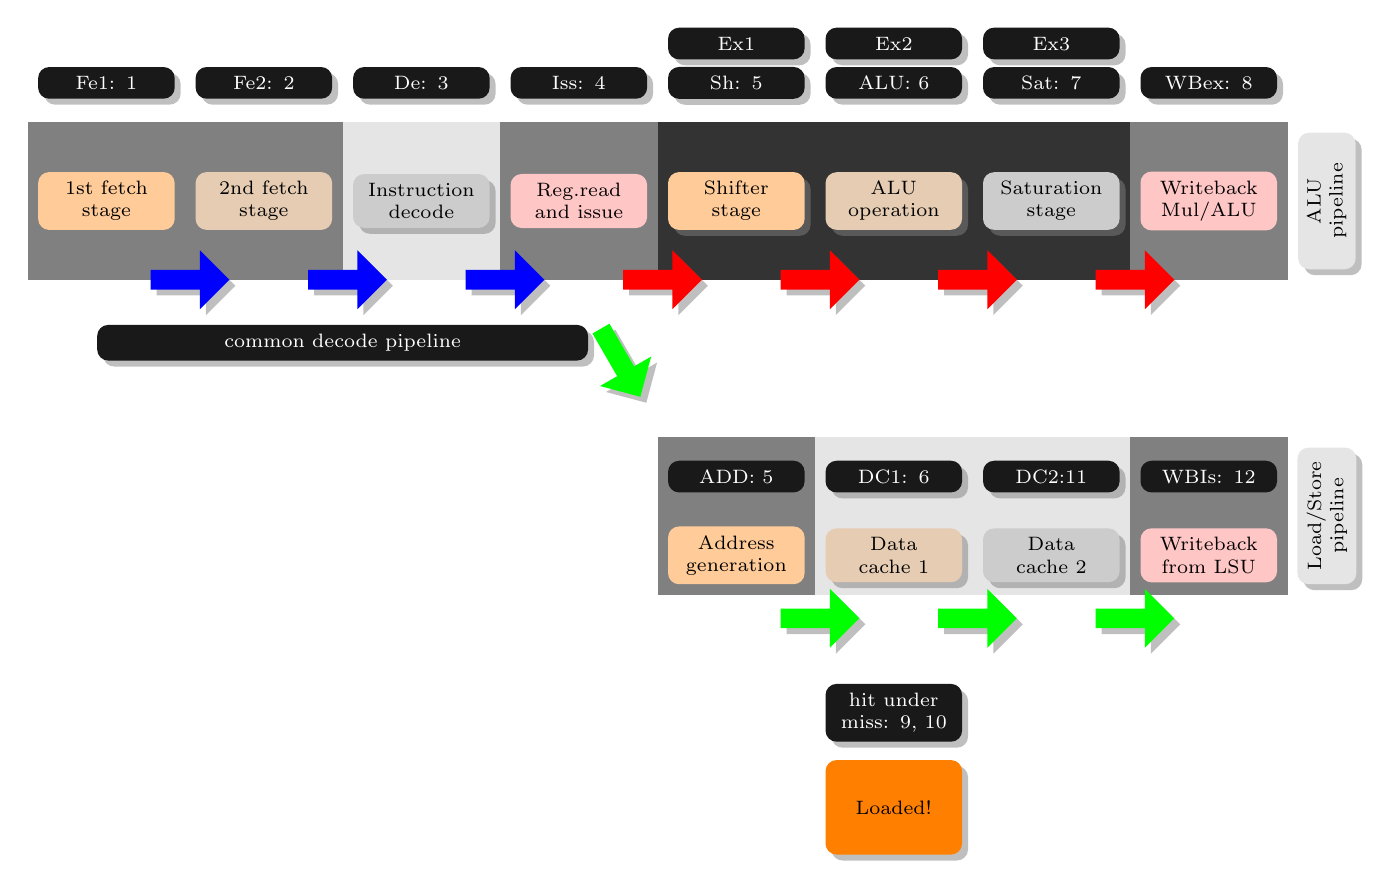
\begin{tikzpicture}
%Arrows
\node[arrow2](ar1) at (-7,-1){};
\node[arrow2](ar2) at (-5,-1){};
\node[arrow2](ar3) at (-3,-1){};
\node[arrow1](ar4) at (-1,-1){};
\node[arrow1](ar5) at ( 1,-1){};
\node[arrow1](ar6) at ( 3,-1){};
\node[arrow1](ar7) at ( 5,-1){};
\node[arrow4](ar8) at ( -1.5,-2){};
\node[arrow3](ar9) at (1,-5.3){}; 
\node[arrow3](ar9) at (3,-5.3){}; 
\node[arrow3](ar9) at (5,-5.3){}; 


%Row One
\node[stage2,rotate=90](alup) at (7.5,0){ALU pipeline};
\node[stage2,rotate=90](lsp) at (7.5,-4){Load/Store pipeline};
\node[stage3](cdp) at (-5,-1.8){common decode pipeline};
\node[stage] (e1) at (0,2){Ex1};
\node[stage] (e2) at (2,2){Ex2};
\node[stage] (e3) at (4,2){Ex3};
\node[stage] (s1) at (-8,1.5){Fe1: 1};
\node[box1] (bx1) at (-8,0){1st fetch stage};
\node[stage] (s) at (-6,1.5){Fe2: 2};
\node[box2] (bx2) at (-6,0){2nd fetch stage};
\node[stage] (s3) at (-4,1.5){De: 3};
\node[box3] (bx3) at (-4,0){Instruction decode};
\node[stage] (s4) at (-2,1.5){Iss: 4};
\node[box4] (bx4) at (-2,0){Reg.read and issue};
\node[stage] (s5) at (0,1.5){Sh: 5};
\node[box1] (bx5) at (0,0){Shifter stage};
\node[stage] (s6) at (2,1.5){ALU: 6};
\node[box2] (bx6) at (2,0){ALU\\operation};
\node[stage] (s7) at (4,1.5){Sat: 7};
\node[box3] (bx7) at (4,0){Saturation stage};
\node[stage] (s8) at (6,1.5){WBex: 8};
\node[box4] (bx8) at (6,0){Writeback Mul/ALU};
%Row Three
\node[stage] (s3_1) at (0,-3.5){ADD: 5};
\node[box1] (r3bx1) at (0,-4.5){Address generation};
\node[stage] (s3_2) at (2,-3.5){DC1: 6};
\node[box2] (r3bx2) at (2,-4.5){Data cache 1};
\node[stage] (s3_3) at (4,-3.5){DC2:11};
\node[box3] (r3bx3) at (4,-4.5){Data cache 2};
\node[stage] (s3_4) at (6,-3.5){WBIs: 12};
\node[box4] (r3bx4) at (6,-4.5){Writeback from LSU};
\node[stage] (s3_4) at (2,-6.5){hit under miss: 9, 10};
\node[box5] (r3bx2) at (2,-7.7){Loaded!};
%background
\begin{scope}[on background layer]
\fill[black!50](-9,-1) rectangle(-5,1);
\end{scope}

\begin{scope}[on background layer]
\fill[black!10](-5,-1) rectangle(-3,1);
\end{scope}

\begin{scope}[on background layer]
\fill[black!50](-3,-1) rectangle(-1,1);
\end{scope}

\begin{scope}[on background layer]
\fill[black!80](-1,-1) rectangle(5,1);
\end{scope}

\begin{scope}[on background layer]
\fill[black!50](-1,-5) rectangle(1,-3);
\end{scope}

\begin{scope}[on background layer]
\fill[black!10](1,-5) rectangle(5,-3);
\end{scope}


\begin{scope}[on background layer]
\fill[black!50](5,-1) rectangle(7,1);
\end{scope}

\begin{scope}[on background layer]
\fill[black!50](5,-5) rectangle(7,-3);
\end{scope}

\end{tikzpicture}
\caption{ARM1176JZF-S Example LDR miss}
\end{figure}
\clearpage
\printbibliography

\end{document}


